\chapter{PHƯƠNG PHÁP NGHIÊN CỨU ĐỀ XUẤT}
\label{ch:proposed_method}

\section{Mô Hình Tổng Quát (System Models)}
\label{sec:system_models}

\subsection{Kiến Trúc Tổng Thể Của Khung RA-HE-DLinear}
Để giải quyết đồng thời các thách thức về tính phi dừng do thay đổi chế độ thị trường, tương quan lan tỏa liên quốc gia và sự vi phạm các ràng buộc nghiệp vụ kinh tế, đồ án đề xuất khung mô hình toàn diện \textbf{RA-HE-DLinear} (\textit{Regime-Aware Hierarchical-Economic DLinear}). 

Kiến trúc tổng thể của hệ thống được mô tả trực quan trong Hình \ref{fig:ra_he_dlinear_architecture}. Hệ thống bao gồm 5 tầng thành phần phối hợp chặt chẽ theo luồng xử lý khép kín:
\begin{enumerate}
    \item \textbf{Tầng tiền xử lý và suy diễn chế độ thị trường (Regime Inference):} Tiếp nhận các chuỗi kinh tế vĩ mô và chỉ số tăng trưởng, huấn luyện mô hình Markov ẩn (HMM) để suy diễn phân phối xác suất hậu nghiệm của các trạng thái thị trường $\bm{\pi}_t = [P(s_t = 1), P(s_t = 2), P(s_t = 3)]^\top$.
    \item \textbf{Tầng bóc tách nhân tố liên quốc gia (Cross-Country TRMF):} Sử dụng thuật toán phân rã ma trận điều chuẩn theo thời gian TRMF để bóc tách các nhân tố tiềm ẩn chung $\mathbf{Z} \in \mathbb{R}^{T \times r}$ và ma trận nhúng không gian $\mathbf{W} \in \mathbb{R}^{N \times r}$, phản ánh các mẫu biến động chung và hiệu ứng lan tỏa xuyên biên giới giữa các thị trường du lịch liên kết.
    \item \textbf{Động cơ thời gian thích ứng chế độ RA-Exo-DLinear:} Mở rộng kiến trúc DLinear bằng cách áp dụng cơ chế FiLM điều biến nhánh xu thế theo vector xác suất $\bm{\pi}_t$, phân rã nhánh mùa vụ và bổ sung các nhánh ánh xạ tham số học được cho biến ngoại sinh lịch nghỉ lễ $\mathbf{X}_{\text{cal}}$ cùng biến kinh tế vĩ mô $\mathbf{X}_{\text{macro}}$.
    \item \textbf{Tầng hiệu chỉnh chiếu mốc neo ràng buộc kinh tế ($\Pi_{\mathcal{C}}$):} Tiếp nhận dự báo thô hai biến mục tiêu $(\hat{Y}_{\text{arr}}, \hat{Y}_{\text{nig}})$, áp dụng toán tử chiếu mốc neo giải tích dạng đóng để loại bỏ triệt để $100\%$ các trường hợp vi phạm cận vật lý $\hat{Y}_{\text{nig}} < \hat{Y}_{\text{arr}}$, đồng thời điều chỉnh tỷ lệ lưu trú $\widehat{\text{LOS}}$ quay trở về dải phân vị kinh tế lịch sử của quốc gia.
    \item \textbf{Tầng lượng hóa độ bất định Conformal (DCQF):} Dự báo đồng thời các phân vị biên $[P_{10}, P_{50}, P_{90}]$ và áp dụng hiệu chuẩn Conformal Prediction để thiết lập dải dự báo tin cậy có bảo đảm toán học trên mẫu hữu hạn.
\end{enumerate}

\begin{figure}[H]
\centering
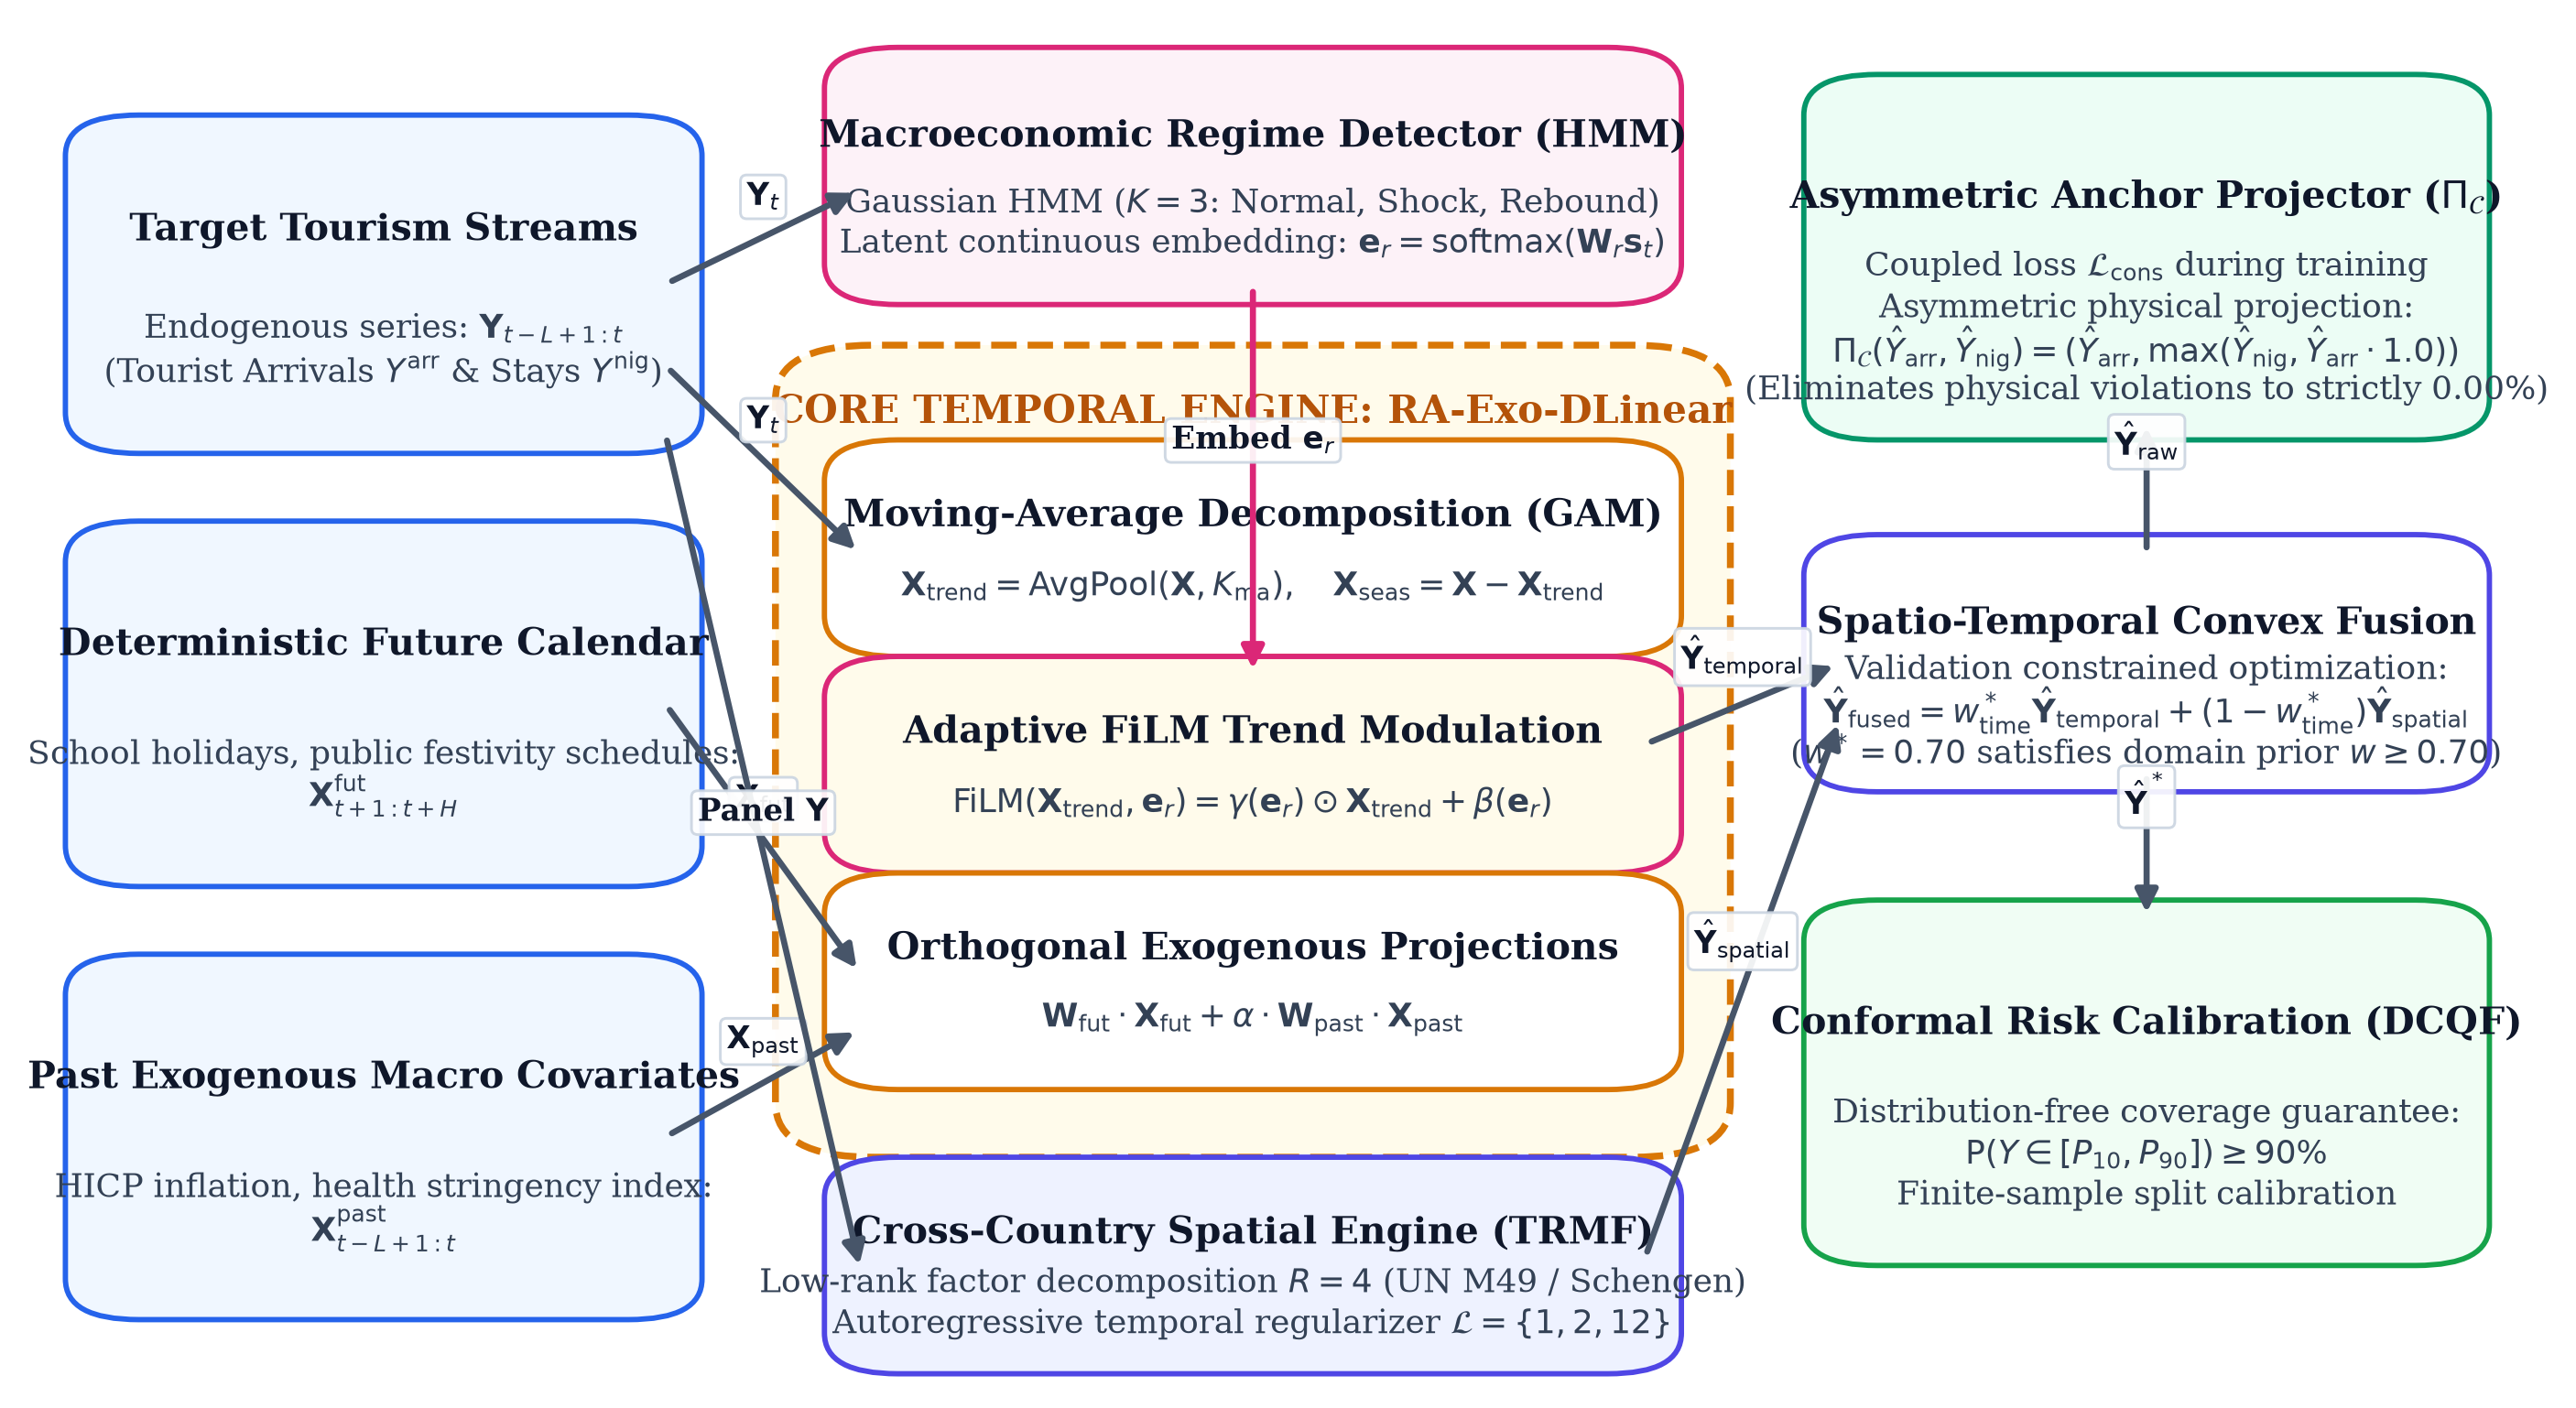
\includegraphics[width=0.98\textwidth]{figures/ra_he_dlinear_architecture.png}
\caption{Kiến trúc tổng thể của khung dự báo RA-HE-DLinear}
\label{fig:ra_he_dlinear_architecture}
\end{figure}

\subsection{Luồng Dữ Liệu và Quy Trình Dự Báo Đa Tầng}
Quy trình vận hành từ đầu vào thô đến kết quả dự báo tin cậy cuối cùng trải qua các bước chuẩn hóa nghiêm ngặt:
\begin{equation}
    \mathbf{X}_{1:t} \xrightarrow{\text{Phân rã \& Ngoại sinh}} \left\{ \mathbf{X}_{\text{trend}}, \mathbf{X}_{\text{seasonal}}, \mathbf{X}_{\text{cal}}, \mathbf{X}_{\text{macro}}, \mathbf{Z}_{\text{trmf}} \right\} \xrightarrow{\text{RA-Exo-DLinear}} \hat{\mathbf{Y}}_{\text{raw}} \xrightarrow{\Pi_{\mathcal{C}}} \hat{\mathbf{Y}}_{\text{cons}} \xrightarrow{\text{DCQF}} \left[ \hat{\mathbf{Y}}^{P_{10}}, \hat{\mathbf{Y}}^{P_{90}} \right]
\end{equation}

\subsection{Ký Hiệu Toán Học và Các Giả Thuyết Nghiên Cứu}
Bảng \ref{tab:math_notations} tổng hợp các ký hiệu toán học chính được sử dụng xuyên suốt đồ án.

\begin{table}[H]
\centering
\caption{Bảng quy ước ký hiệu toán học}
\label{tab:math_notations}
\begin{tabular}{ll}
\toprule
\textbf{Ký hiệu} & \textbf{Ý nghĩa định nghĩa} \\
\midrule
$N$ & Số lượng quốc gia hoặc nền kinh tế quan trắc ($N=38$ với Eurostat, $N=203$ với World Bank) \\
$T$ & Tổng số mốc thời gian quan sát trong tập dữ liệu \\
$L$ & Chiều dài cửa sổ quan sát lịch sử ($L=24$ tháng đối với dữ liệu tháng) \\
$H$ & Chân trời dự báo tương lai ($H \in \{3, 6, 12\}$ tháng) \\
$Y_{\text{arr}, i, t}$ & Số lượt khách du lịch đến quốc gia $i$ tại thời điểm $t$ \\
$Y_{\text{nig}, i, t}$ & Số đêm lưu trú tại cơ sở lưu trú của quốc gia $i$ tại thời điểm $t$ \\
$\text{LOS}_{i, t}$ & Thời gian lưu trú trung bình: $\text{LOS}_{i, t} = Y_{\text{nig}, i, t} / Y_{\text{arr}, i, t}$ \\
$\mathbf{X}_{\text{cal}}$ & Ma trận biến ngoại sinh lịch lễ đã biết trước trong tương lai \\
$\mathbf{X}_{\text{macro}}$ & Ma trận biến ngoại sinh kinh tế vĩ mô trễ trong quá khứ \\
$\bm{\pi}_t$ & Vector xác suất hậu nghiệm chế độ thị trường từ HMM tại thời điểm $t$ \\
$\mathbf{Z}_t, \mathbf{W}$ & Nhân tố tiềm ẩn thời gian và ma trận trọng số không gian của TRMF \\
$\Pi_{\mathcal{C}}$ & Toán tử chiếu mốc neo bảo đảm ràng buộc kinh tế \\
$\mathcal{L}_{\text{cons}}$ & Hàm mất mát phạt vi phạm ràng buộc liên kết \\
\bottomrule
\end{tabular}
\end{table}

\noindent \textbf{Các giả thuyết nghiên cứu chính:}
\begin{itemize}
    \item \textbf{Giả thuyết H1 (Tính thích ứng chế độ):} Việc điều biến nhánh xu thế tuyến tính bằng cơ chế FiLM phụ thuộc vào trạng thái HMM sẽ làm giảm đáng kể sai số dự báo trong các giai đoạn đứt gãy cấu trúc so với mô hình tuyến tính tĩnh.
    \item \textbf{Giả thuyết H2 (Hiệu ứng lan tỏa liên quốc gia):} Việc bổ sung biểu diễn nhân tố tiềm ẩn TRMF cho phép mô hình khai thác hiệu quả các dao động chung khu vực, cải thiện độ chính xác dự báo so với tiếp cận dự báo độc lập từng quốc gia.
    \item \textbf{Giả thuyết H3 (Tính nhất quán miền):} Việc áp dụng toán tử chiếu mốc neo $\Pi_{\mathcal{C}}$ bảo đảm loại bỏ hoàn toàn vi phạm vật lý mà không làm méo mó phân phối hoặc suy giảm độ chính xác tổng thể.
\end{itemize}

\section{Phương Pháp Nghiên Cứu Đề Xuất (Proposed Approaches)}
\label{sec:proposed_approaches}

\subsection{Động Cơ Chuỗi Thời Gian RA-Exo-DLinear}
\label{subsec:ra_exo_dlinear}
Động cơ thời gian cốt lõi của hệ thống mở rộng kiến trúc DLinear cổ điển theo hướng tích hợp đa thành phần biến đổi học được:

\subsubsection{Phân Rã Chuỗi Đa Kênh Bằng Bộ Lọc Trung Bình Trượt}
Chuỗi quan trắc lịch sử độ dài $L$ của biến mục tiêu (lượt khách hoặc số đêm) được phân rã thành hai thành phần cơ sở:
\begin{align}
    \mathbf{X}_{\text{trend}} &= \text{AvgPool}(\text{Pad}(\mathbf{X}, k_{\text{ma}})) \in \mathbb{R}^{L} \\
    \mathbf{X}_{\text{seasonal}} &= \mathbf{X} - \mathbf{X}_{\text{trend}} \in \mathbb{R}^{L}
\end{align}

\subsubsection{Cơ Chế FiLM Điều Biến Nhánh Xu Thế Theo Trạng Thái HMM}
Đối với nhánh xu thế, thay vì sử dụng ánh xạ affine cố định, mô hình tính toán các tham số điều biến động $\bm{\gamma} \in \mathbb{R}^H$ và $\bm{\beta} \in \mathbb{R}^H$ từ vector xác suất trạng thái thị trường $\bm{\pi}_t \in \mathbb{R}^K$:
\begin{align}
    \bm{\gamma}(\bm{\pi}_t) &= \mathbf{W}_{\gamma} \bm{\pi}_t + \mathbf{b}_{\gamma} \\
    \bm{\beta}(\bm{\pi}_t)  &= \mathbf{W}_{\beta} \bm{\pi}_t + \mathbf{b}_{\beta}
\end{align}
Dự báo nhánh xu thế ban đầu được tạo ra bởi ma trận trọng số $\mathbf{W}_{\text{trend}} \in \mathbb{R}^{H \times L}$, sau đó được điều biến bởi FiLM:
\begin{equation}
    \hat{\mathbf{Y}}_{\text{trend}} = \bm{\gamma}(\bm{\pi}_t) \odot \left( \mathbf{W}_{\text{trend}} \mathbf{X}_{\text{trend}} \right) + \bm{\beta}(\bm{\pi}_t) + \mathbf{b}_{\text{trend}}
\end{equation}
Cơ chế này cho phép mô hình: khi thị trường bước vào trạng thái khủng hoảng ($P(s_t = \text{Crisis}) \approx 1$), $\bm{\gamma}$ tự động giảm xuống dưới $1{,}0$ và $\bm{\beta} < 0$ để làm phẳng độ dốc xu thế tăng trưởng quá khứ, ngăn ngừa việc dự báo quá lạc quan.

\subsubsection{Nhánh Mùa Vụ và Các Nhánh Ngoại Sinh Học Được}
\begin{itemize}
    \item \textbf{Nhánh mùa vụ:} Duy trì ánh xạ tuyến tính trực tiếp để bảo toàn các chu kỳ dao động định kỳ:
    \begin{equation}
        \hat{\mathbf{Y}}_{\text{seasonal}} = \mathbf{W}_{\text{seasonal}} \mathbf{X}_{\text{seasonal}} + \mathbf{b}_{\text{seasonal}}
    \end{equation}
    \item \textbf{Nhánh biến ngoại sinh lịch lễ đã biết trước:} Tiếp nhận ma trận biến lịch lễ trong tương lai $\mathbf{X}_{\text{cal}} \in \mathbb{R}^{H \times d_{\text{cal}}}$ (số ngày lễ, số ngày cuối tuần trong $H$ tháng tới):
    \begin{equation}
        \hat{\mathbf{Y}}_{\text{cal}} = \sum_{j=1}^{d_{\text{cal}}} \mathbf{w}_{\text{cal}, j} \odot \mathbf{X}_{\text{cal}, :, j} + \mathbf{b}_{\text{cal}}
    \end{equation}
    \item \textbf{Nhánh biến kinh tế vĩ mô trễ:} Tiếp nhận biến kinh tế trễ trong quá khứ $\mathbf{X}_{\text{macro}} \in \mathbb{R}^{L \times d_{\text{macro}}}$:
    \begin{equation}
        \hat{\mathbf{Y}}_{\text{macro}} = \mathbf{W}_{\text{macro}} \text{vec}(\mathbf{X}_{\text{macro}}) + \mathbf{b}_{\text{macro}}
    \end{equation}
    \item \textbf{Nhánh nhân tố liên quốc gia TRMF:} Tiếp nhận vector nhúng không gian $\mathbf{w}_i \in \mathbb{R}^r$ và dự báo nhân tố tiềm ẩn tương lai $\hat{\mathbf{Z}}_{t+1:t+H} \in \mathbb{R}^{H \times r}$:
    \begin{equation}
        \hat{\mathbf{Y}}_{\text{trmf}} = \hat{\mathbf{Z}}_{t+1:t+H} \mathbf{w}_i
    \end{equation}
\end{itemize}

Dự báo thô tổng hợp của mô hình là tổng tuyến tính của toàn bộ các nhánh:
\begin{equation}
    \hat{\mathbf{Y}}_{\text{raw}} = \hat{\mathbf{Y}}_{\text{trend}} + \hat{\mathbf{Y}}_{\text{seasonal}} + \hat{\mathbf{Y}}_{\text{cal}} + \hat{\mathbf{Y}}_{\text{macro}} + \hat{\mathbf{Y}}_{\text{trmf}}
\end{equation}

\subsection{Toán Tử Chiếu Mốc Neo Ràng Buộc Kinh Tế $\Pi_{\mathcal{C}}$}
\label{subsec:projection_operator}
Sau khi thu được cặp dự báo thô $\hat{\mathbf{Y}}_{\text{raw}} = [\hat{Y}_{\text{arr}}, \hat{Y}_{\text{nig}}]^\top$, mô hình áp dụng toán tử chiếu mốc neo để bảo đảm hai cấp độ ràng buộc nghiệp vụ:

\subsubsection{Cấp Độ 1: Bảo Đảm Cận Vật Lý Không Thể Phá Vỡ}
Theo định nghĩa, số đêm lưu trú phải luôn lớn hơn hoặc bằng số lượt khách: $\hat{Y}_{\text{nig}} \ge \hat{Y}_{\text{arr}}$. Vì lượt khách được kiểm đếm với độ chính xác cao tại cửa khẩu, ta giữ $\hat{Y}_{\text{arr}}$ làm mốc neo chuẩn và thực hiện phép chiếu cận dưới lên số đêm lưu trú:
\begin{equation}
    \hat{Y}_{\text{nig}}^{(1)} = \max\left( \hat{Y}_{\text{nig}}, \; \hat{Y}_{\text{arr}} \right)
\end{equation}
Công thức giải tích đơn giản này bảo đảm triệt để rằng sau phép chiếu, tỷ lệ vi phạm vật lý luôn bằng chính xác $0\%$.

\subsubsection{Cấp Độ 2: Bảo Đảm Tính Nhất Quán Theo Dải Kinh Tế Lịch Sử}
Mỗi quốc gia có đặc thù du lịch riêng: các quốc gia du lịch biển đảo (như Hy Lạp, Tây Ban Nha, Croatia) có thời gian lưu trú trung bình dài ($\text{LOS} \in [3{,}0, 6{,}5]$), trong khi các quốc gia du lịch công vụ hoặc trung chuyển ngắn ngày (như Luxembourg, Bỉ) có $\text{LOS} \in [1{,}2, 2{,}5]$.

Dựa trên dữ liệu lịch sử trong cửa sổ huấn luyện của quốc gia $i$, ta xác định dải phân vị kinh tế thực nghiệm của tỷ lệ lưu trú: $[r_{\min, i}, r_{\max, i}] = [Q_{0{,}05}(\text{LOS}_i), Q_{0{,}95}(\text{LOS}_i)]$. Khi đó, dự báo số đêm lưu trú được chiếu nhẹ vào dải phân vị kinh tế:
\begin{equation}
    \hat{Y}_{\text{nig}}^{(2)} = \text{clip}\left( \hat{Y}_{\text{nig}}^{(1)}, \; r_{\min, i} \cdot \hat{Y}_{\text{arr}}, \; r_{\max, i} \cdot \hat{Y}_{\text{arr}} \right)
\end{equation}

\subsubsection{Hàm Mất Mát Phạt Ràng Buộc Liên Kết ($\mathcal{L}_{\text{cons}}$)}
Để mô hình nơ-ron chủ động học được cấu trúc tương quan này ngay trong quá trình lan truyền ngược mà không chỉ phụ thuộc vào phép chiếu hậu kỳ, ta bổ sung số hạng phạt vi phạm liên kết vào hàm mất mát huấn luyện:
\begin{equation}
    \mathcal{L}_{\text{cons}} = \frac{1}{H} \sum_{h=1}^H \text{ReLU}\left( \hat{Y}_{\text{arr}, t+h} - \hat{Y}_{\text{nig}, t+h} \right)^2 + \lambda_{\text{band}} \left[ \text{ReLU}\left( r_{\min} \hat{Y}_{\text{arr}} - \hat{Y}_{\text{nig}} \right)^2 + \text{ReLU}\left( \hat{Y}_{\text{nig}} - r_{\max} \hat{Y}_{\text{arr}} \right)^2 \right]
\end{equation}

\subsection{Lượng Hóa Độ Bất Định Bằng Deep Conformal Quantile Forecasting}
\label{subsec:conformal_prediction}
Để cung cấp dải dự báo tin cậy $[P_{10}, P_{90}]$, kiến trúc đầu ra của mô hình dự báo đồng thời ba giá trị phân vị $\hat{q}_{\tau}$ với $\tau \in \{0{,}10, \; 0{,}50, \; 0{,}90\}$ thông qua hàm mất mát Pinball Loss (Quantile Loss):
\begin{equation}
    \mathcal{L}_{\text{pinball}}(y, \hat{q}_\tau) = \max\left( \tau (y - \hat{q}_\tau), \; (1 - \tau) (\hat{q}_\tau - y) \right)
\end{equation}

Sau đó, trên tập dữ liệu hiệu chuẩn gồm $M$ mẫu độc lập $\mathcal{D}_{\text{cal}} = \{(\mathbf{x}_m, y_m)\}_{m=1}^M$, ta tính toán điểm không tương đồng Conformal (\textit{conformity score}) cho từng mẫu:
\begin{equation}
    s_m = \max\left( \hat{q}_{0{,}10}(\mathbf{x}_m) - y_m, \; y_m - \hat{q}_{0{,}90}(\mathbf{x}_m) \right)
\end{equation}
Gọi $\hat{s}_{1-\alpha}$ là giá trị phân vị bậc $\lceil (M + 1)(1 - \alpha) \rceil / M$ của tập hợp điểm sai số $\{s_m\}_{m=1}^M$. Khi đó, khoảng dự báo Conformal hiệu chỉnh cho mẫu thử nghiệm mới $\mathbf{x}_{\text{test}}$ được xác lập bởi:
\begin{equation}
    \hat{C}_{1-\alpha}(\mathbf{x}_{\text{test}}) = \left[ \hat{q}_{0{,}10}(\mathbf{x}_{\text{test}}) - \hat{s}_{1-\alpha}, \; \hat{q}_{0{,}90}(\mathbf{x}_{\text{test}}) + \hat{s}_{1-\alpha} \right]
\end{equation}
Định lý Conformal Prediction bảo đảm rằng:
\begin{equation}
    P\left( Y_{\text{test}} \in \hat{C}_{1-\alpha}(\mathbf{x}_{\text{test}}) \right) \ge 1 - \alpha
\end{equation}

\subsection{Thuật Toán Tối Ưu Hóa Liên Hợp (Coupled Optimizer)}
\label{subsec:coupled_optimizer}
Quá trình huấn luyện toàn bộ hệ thống được thực hiện liên hợp thông qua thuật toán được trình bày chi tiết trong Khối Thuật toán \ref{alg:coupled_optimizer}.

\begin{algorithm}[H]
\caption{Thuật toán huấn luyện liên hợp RA-HE-DLinear (Coupled Optimizer)}
\label{alg:coupled_optimizer}
\begin{algorithmic}[1]
\REQUIRE Bảng dữ liệu chuỗi thời gian đa quốc gia $\mathbf{Y}$, biến ngoại sinh lịch lễ $\mathbf{X}_{\text{cal}}$, biến vĩ mô $\mathbf{X}_{\text{macro}}$, độ dài lịch sử $L$, chân trời $H$, tốc độ học $\eta$, trọng số phạt $\lambda_{\text{cons}}$.
\ENSURE Các tham số mô hình tối ưu $\bm{\Theta}^*$ và tham số hiệu chuẩn Conformal $\hat{s}_{1-\alpha}$.
\STATE \textbf{Bước 1: Huấn luyện HMM và TRMF trước}
\STATE Ước lượng mô hình Markov ẩn 3 trạng thái trên biến động kinh tế $\mathbf{u}_{1:T}$ bằng giải thuật Baum-Welch, thu được vector phân phối xác suất hậu nghiệm $\bm{\pi}_t$.
\STATE Phân rã ma trận TRMF trên $\mathbf{Y}_{1:T}$ với hạng $r=5$, thu được ma trận không gian $\mathbf{W}$ và chuỗi nhân tố $\mathbf{Z}_{1:T}$.
\STATE \textbf{Bước 2: Huấn luyện mạng RA-Exo-DLinear}
\FOR{mỗi epoch $e = 1, 2, \dots, E_{\max}$}
    \FOR{mỗi mini-batch $(\mathbf{X}_{\text{batch}}, \mathbf{Y}_{\text{batch}})$}
        \STATE Phân rã xu thế và mùa vụ: $\mathbf{X}_{\text{trend}}, \mathbf{X}_{\text{seasonal}} \leftarrow \text{Decompose}(\mathbf{X}_{\text{batch}})$
        \STATE Điều biến FiLM nhánh xu thế: $\hat{\mathbf{Y}}_{\text{trend}} \leftarrow \bm{\gamma}(\bm{\pi}_t) \odot (\mathbf{W}_{\text{trend}} \mathbf{X}_{\text{trend}}) + \bm{\beta}(\bm{\pi}_t)$
        \STATE Tính toán các nhánh: $\hat{\mathbf{Y}}_{\text{seasonal}}, \hat{\mathbf{Y}}_{\text{cal}}, \hat{\mathbf{Y}}_{\text{macro}}, \hat{\mathbf{Y}}_{\text{trmf}}$
        \STATE Tổng hợp dự báo thô: $\hat{\mathbf{Y}}_{\text{raw}} = \hat{\mathbf{Y}}_{\text{trend}} + \hat{\mathbf{Y}}_{\text{seasonal}} + \hat{\mathbf{Y}}_{\text{cal}} + \hat{\mathbf{Y}}_{\text{macro}} + \hat{\mathbf{Y}}_{\text{trmf}}$
        \STATE Tính hàm mất mát tổng hợp:
        \STATE $\quad \mathcal{L}_{\text{total}} = \mathcal{L}_{\text{pinball}}(\mathbf{Y}, \hat{\mathbf{Y}}_{\text{raw}}) + \lambda_{\text{cons}} \mathcal{L}_{\text{cons}}(\hat{\mathbf{Y}}_{\text{raw}})$
        \STATE Cập nhật trọng số bằng thuật toán AdamW: $\bm{\Theta} \leftarrow \bm{\Theta} - \eta \nabla_{\bm{\Theta}} \mathcal{L}_{\text{total}}$
    \ENDFOR
\ENDFOR
\STATE \textbf{Bước 3: Hiệu chuẩn Conformal Prediction}
\STATE Tính toán điểm không tương đồng $\{s_m\}_{m=1}^M$ trên tập hiệu chuẩn $\mathcal{D}_{\text{cal}}$.
\STATE Xác định ngưỡng phân vị $\hat{s}_{1-\alpha} \leftarrow \text{Quantile}(\{s_m\}, 1 - \alpha)$.
\RETURN Mô hình tối ưu $\bm{\Theta}^*$ và ngưỡng $\hat{s}_{1-\alpha}$.
\end{algorithmic}
\end{algorithm}
